\chapter{Теоретичні відомості}

%%===========================================================================%%
\section{Знаходження глибини методом бінокулярного паралаксу}
%%===========================================================================%%
\subsection{Будова камери}
Сучасні цифрові фото та відео камери мають куди більш складну будову ніж їх попередники. Для подальших викладок нам буде достатньо розглянути роботу найпростішої можливої камери --- камери-обскури (від лат. camera obscūra — «темна кімната») (рис. \ref{1.1.1 - Camera-obscura}). Це просто темне приміщення з одним малим отвором, через який на протилежну стіну проектується перевернуте зображення предметів ззовні. Тільки зараз протилежна стіна --- матриця цифрової камери. 
\begin{figure}[h!]
	\centering
	\includegraphics[scale = 0.5]{CO2.pdf}
	\caption{Камера-обскура}
	\label{1.1.1 - Camera-obscura}
\end{figure}


%%---------------------------------------------------------------------------%%
\subsection{Пошук відстані методом бінокулярного паралаксу}
В силу оптичних особливостей результуюче зображення в камерi-обскурі буде перевернутим. Тому для більшого спрощення перенесемо матрицю камери вправо від, на відстань $f$. Це ніяк не вплине на результат, але сильно спростить подальші викладки.

Покажемо тепер, як з допомогою двох таких камер можна знайти абсолютну відстань до об'єкта. Камери розташовані паралельно одна одній.
Тоді маємо таку конфігурацію (рис. \ref{geometry}).%\newline
\begin{figure}[!htb]
	\centering
	\includegraphics[scale = 0.6]{geometry.pdf}
	\caption{Геометрія розташування камер}
	\label{geometry}
\end{figure}
Тут $f$ --- фокусна відстань, $z$ --- відстань до об'єкта, $\Delta$ --- відстань між камерами, $x_1$ та $x_2$ --- координати об'єкта на лівому та правому знімках. $R, L$ --- оптичні центри правої и лівої камери, $S$ --- об'єкт.

Тоді з подібності трикутників $LSL' , Lx_1O_L$ та $RSR' , Rx_2O_R$ (!) маємо:
$$\begin{cases} \frac{f}{x_1} = \frac{z}{\Delta + x} , \\ \frac{f}{x_2} = \frac{z}{x} . \end{cases}$$
	
Виразивши $\Delta$ з першого рівняння та $x$ з другого, отримаємо:
$$\begin{cases} \Delta = \frac{z \cdot x_1}{f} - x , \\ x = \frac{z \cdot x_2}{f} . \end{cases}$$
	
Підставимо $x$ в перше рівняння і отримаємо вираз для $z$:
$$ z = \frac{\Delta \cdot f}{(x_1 - x_2)} .$$
	
Оскільки $\Delta$ и $f$ не залежать від розташування об'єкта, то відстань до нього буде залежати тільки від різниці $x_1 - x_2$, тобто тільки від зсуву об'єкту між двома знімками. Тож для знаходження глибини сцени нам необхідно знайти зсув для кожного пікселя між зображеннями.
	


%%===========================================================================%%
\section{Оффлайн алгоритм пошуку скалярного поля зсувів}\label{offline}
%%===========================================================================%%
\subsection{Постановка задачі}
Далі під зображенням будемо розуміти деякий рядок вихідного зображення.

Нехай $n$ --- довжина зображення, $I = \{1, 2, .., n\}$ --- множина координат пікселів, $D = \{0, ... , D_{max}\}$ ---  множина зсувів, де $D_{max}$ --- значення максимального зсуву, що обирається емпіричним шляхом. 
Ліве і праве зображення задамо як функції
\begin{align*}
	\mathcal{L} &: I \rightarrow \mathcal{C} , \\
	\mathcal{R} &: I \rightarrow \mathcal{C} .
\end{align*}
Тобто, $\mathcal{L}(i)$ --- інтенсивність $i$-го пікселя на лівому зображені, а $\mathcal{R}(i)$ --- інтенсивність $i$-го пікселя на правому зображені, а $ \mathcal{C} $ --- множина кольорів зображення.

Для вирішення задачі кожному пікселю лівого зображення потрібно знайти відповідний йому піксель на правому зображенні (\ref{mapping}). Введемо сюр'єктивне відображення $ d : I \rightarrow D $, де $ d(i) $ --- такий зсув $ d_i \in D$ для пікселя з номером $i$ лівого зображення, що піксель правого зображення  з номером $i - d_i$ відповідав йому.
%mapping
\begin{figure}[h!]
	\centering
	\includegraphics[scale = 1]{mapping.pdf}
	\caption{Пошук відповідних пікселів}
	\label{mapping}
\end{figure}
Проте, не будь-яка пара пікселів може знаходитися у відповідності --- пікселю з номером $i$ на лівому зображені можуть відповідати тільки ті пікселі  правого зображення з номером $j$, для яких $i \leq j$. Переконатися в цьому можна тримаючи перед собою олівець, та по черзі закриваючи то праве, то ліве око. Для правого ока олівець буде знаходитися лівіше ніж для лівого

Треба знайти таку послідовність $\overline{d} \in {D}^n$, яка б мінімізувала штрафну функцію
\begin{equation}
	\mathcal{W}(\overline{d}) = \sum\limits_{i = 1}^n h(i, d_i) + \sum\limits_{i = 1}^{n-1} g(d_i, d_{i + 1}),
\end{equation}
\label{penalty}
де $ h(i, d_i) $ відповідає за схожість кольору пікселів, а $ g(d_i, d_{i + 1}) $ за гладкість поля зсувів.


%%---------------------------------------------------------------------------%%
\subsection{Представлення задачі як пошук найкоротшого шляху у графі}\label{offline_graph}
Зведемо задачу пошуку послідовності $ \overline{d} $ , що мінімізує штрафну функцію (\ref{penalty}), як пошук найкоротшого шляху через орієнтований зважений граф $G = <\mathcal{V}, \mathcal{E}>$ (\ref{graphG}).
Його множина вершин 
$$ \mathcal{V} = \{ \sigma(i, d) \, | \, i \in I, \, d \in D \} \cup \{ S, E \} .$$
Кожна вершина $\sigma(i, d)$ має вагу $h(i, d) \;, \; \forall i \in I, \, d \in D .$ Множина його ребер
$$ \mathcal{E} = \bigcup\limits_{d \in D }<S, \sigma(1, d) > \; \cup \bigcup\limits_{\substack{d \in D}} <\sigma(n, d), E > \; \cup 
\bigcup\limits_{\substack{i = 1..n-1 \\d \in D \\d' \in D}} <\sigma(i, d), \sigma(i+1, d') >.$$
Введемо функцію ваг ребер 
$$ w : \mathcal{E} \rightarrow \mathbb{R}, $$
де $ w(v_1, v_2) $ ---  вага ребра $ <v_1, v_2>, \; v_1, v_2 \in \mathcal{V} $.
Тоді
\begin{itemize}
\item  $ w(S,  \sigma(1, d) ) = 0 $, $ \forall d \in D $
\item  $ w(\sigma(n, d), E ) = 0 $, $ \forall d \in D $
\item  $ w(\sigma(i, d), \sigma(i + 1, d ') ) = g(d, d') $, $ \; \forall d, d' \in D, i \in I $
\end{itemize}

\begin{figure}[h!]
	\centering
	\tikzset{>=latex}
	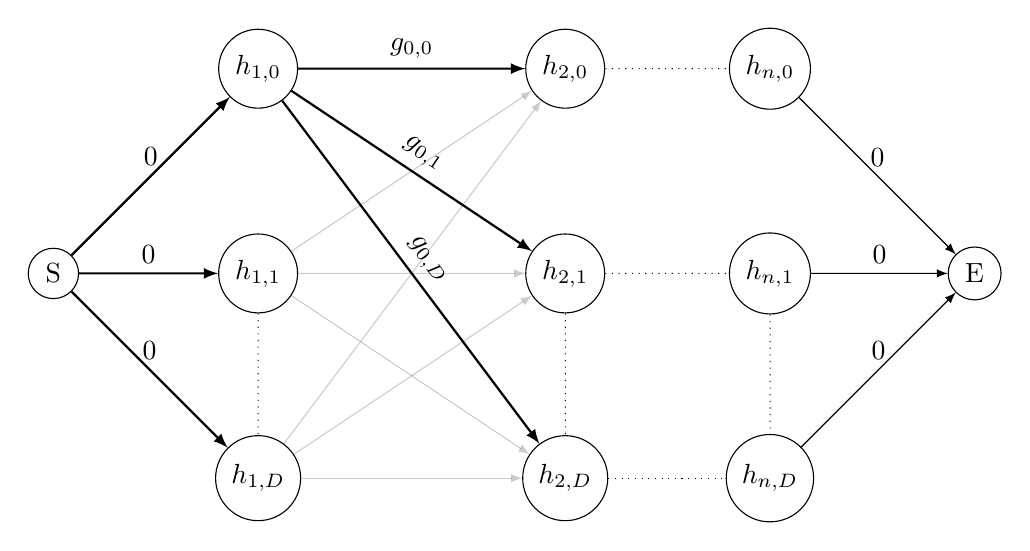
\begin{tikzpicture}[scale=1.3]
	\tikzstyle{vertex} = [circle, draw=black]
	\tikzstyle{edge} = [->, thick]

%----------Виходить такий граф:------------------------------
	\node[vertex] (s) at (0,2) {S};
	
	\node[vertex] (v1n) at (2,0) {$h_{1,D}$};
	\node[vertex] (v11) at (2,2) {$h_{1,1}$};
	\node[vertex] (v10) at (2,4) {$h_{1,0}$};
	
	\path[->, thick] (s) edge node[ above ] {0} (v1n);
	\path[->, thick] (s) edge node[ above ] {0} (v11);
	\path[->, thick] (s) edge node[ above ] {0} (v10);
	
	\draw[dash pattern=on \pgflinewidth off 2pt] (v11)--(v1n);
	
%------------------------------------------------------------
	\node[vertex] (v2n) at (5,0) {$h_{2,D}$};
	\node[vertex] (v21) at (5,2) {$h_{2,1}$};
	\node[vertex] (v20) at (5,4) {$h_{2,0}$};

	\path[->, opacity=0.2] (v11) edge node[ above,sloped ] {} (v2n);
	\path[->, opacity=0.2] (v11) edge node[ above,sloped ] {} (v21);
	\path[->, opacity=0.2] (v11) edge node[ above,sloped ] {} (v20);
	
	\path[->, opacity=0.2] (v1n) edge node[ above,sloped ] {} (v2n);
	\path[->, opacity=0.2] (v1n) edge node[ above,sloped ] {} (v21);
	\path[->, opacity=0.2] (v1n) edge node[ above,sloped ] {} (v20);
	
	%Selected
	\path[->, thick] (v10) edge node[ above,sloped ] {$g_{0,D}$} (v2n);
	\path[->, thick] (v10) edge node[ above,sloped ] {$g_{0,1}$} (v21);
	\path[->, thick] (v10) edge node[ above,sloped ] {$g_{0,0}$} (v20);
	
	\draw[dash pattern=on \pgflinewidth off 2pt] (v21)--(v2n);
	
	
%------------------------------------------------------------
	\node[vertex] (vnn) at (7,0) {$h_{n,D}$};
	\node[vertex] (vn1) at (7,2) {$h_{n,1}$};
	\node[vertex] (vn0) at (7,4) {$h_{n,0}$};


	\draw[dash pattern=on \pgflinewidth off 2pt] (v2n)--(vnn);
	\draw[dash pattern=on \pgflinewidth off 2pt] (v21)--(vn1);
	\draw[dash pattern=on \pgflinewidth off 2pt] (v20)--(vn0);
	
	\draw[dash pattern=on \pgflinewidth off 2pt] (vn1)--(vnn);
%------------------------------------------------------------
	\node[vertex] (e) at (9,2) {E};

	\path[->] (vnn) edge node[ above ] {0} (e);
	\path[->] (vn1) edge node[ above ] {0} (e);
	\path[->] (vn0) edge node[ above ] {0} (e);
	
	\end{tikzpicture}
	\caption{Граф $G$}
	\label{graphG}
\end{figure}


Тоді послідовність $\overline{d}$ --- послідовність вершин, через які проходить найкоротший шлях з $S$ в $E$, яка буде мінімізувати штрафну функцію $ \mathcal{W}(\overline{d}) $ (\ref{penalty}).


%%---------------------------------------------------------------------------%%
\subsection{Пошук найкоротшого шляху у графі}
Позначимо довжину найкоротшого шляху з вершини S в вершину $ \sigma(i, d) $ як $ f_i (d) $. 
Тоді 
\begin{align*}
	f_1 (d) &= h(1, d),  \forall d \in D \\
	f_2 (d) &=  \min\limits_{d' \in D}\Big( f_1(d) + g(d', d) \Big) + h(2, d),  \forall d \in D \\
	&\vdots \\
	f_i (d) &= \min\limits_{d' \in D}\Big( f_{i-1}(d) + g(d', d) \Big) + h(i, d),  \forall d \in D .
\end{align*}
Тоді елементи послідовності $\overline{d}$ знаходимо за формулами:
\begin{align*}
d_n &= \argmin\limits_{d' \in D}{\big( f_n(d') \big)}, \\
d_i &= \argmin\limits_{d' \in D}{\big( f_{i}(d') + g(d',d_{i+1})\big) \; i = \overline{n-1, 1}}
\end{align*}
\newpage



%%===========================================================================%%
\section{Онлайн алгоритм пошуку скалярного поля зсувів}
%%===========================================================================%%
Метод, описаний в частині \ref{offline}, потребує наявності всіх даних до початку обчислень. В ситуації, коли дані надходять повільно, цей метод не є ефективним, адже доводиться чекати надходження всіх даних і тільки потім починати обчислення, адже ми не можемо розрахувати ваги деяких вершин.
Замість цього можна проводити деякі розрахунки з частиною даних що вже надійшла, цим самим зменшивши час роботи алгоритму після отримання всіх даних.

\subsection{Постановка задачі}
Як і в частині \ref{offline}, $n$ --- довжина зображення, $I = \{1, 2, .., n\}$ --- множина координат пікселів, $D = \{0, ... , D_{max}\}$ --- множина зсувів, $D_{max}$ --- значення максимального зсуву. 
Проте ліве і праве зображення вже задаємо як функції 
\begin{align*}
	\mathcal{L} &: I \rightarrow \mathcal{C} \cup \{ \varepsilon \}, \\
	\mathcal{R} &: I \rightarrow \mathcal{C} \cup \{ \varepsilon \}.
\end{align*}

Якщо $i$-й піксель лівого зображення вже надійшов, то $ \mathcal{L}(i) $ --- інтенсивність $i$-го пікселя на лівому зображені. Якщо ще не надійшов, то $ \mathcal{L}(i) =  \varepsilon $.
Так само, як і у \ref{offline}, нам потрібно знайти таку послідовність $\overline{d} \in {D}^n$, яка мінімізує штрафну функцію \ref{penalty}.

Цю задачу ми теж представимо, як пошук найкоротшого шляху на графі $G = <\mathcal{V}, \mathcal{E}>$.
Його множина вершин, множина ребер та ваги ребер такі ж як і в частині \ref{offline_graph}.
Вага вершини $\sigma(i, d) = $ 
$$\begin{cases} h(i,d), $ якщо $  \mathcal{L}(i) \neq  \varepsilon, \\ \infty,  $ якщо $ \mathcal{L}(i) =  \varepsilon. \end{cases}$$

Будемо називати вершину $\sigma(i, d)$ \textbf{відкритою}, якщо $ \mathcal{L}(i) \neq \varepsilon$, інакше назвемо її \textbf{закритою}.

Отже, поки нам не надійшли всі дані, ми не можемо знайти таку послідовність $\overline{d} \in {D}^n$, що мінімізує штрафну функцію
$$\omega(\overline{d}) = \sum\limits_{i = 1}^n h(i, d_i) + \sum\limits_{i = 1}^{n-1} g(d_i, d_{i + 1}).$$ 
Але, щоб зменшити загальний час роботи алгоритму, ми можемо проводити деякі розрахунки з тими даними, що вже надійшли.



%%---------------------------------------------------------------------------%%
\subsection{Поступове упорядковане надходження даних}
Нехай на початку нам не відомі жодні пікселі обох зображень (рис. \ref{2.1nodata}),
\begin{figure}[h!]
	\centering
	\includegraphics[scale = 0.8]{allclosed2.pdf}
	\caption{Немає даних}
	\label{2.1nodata}
\end{figure}
та існує деякий стохастичний автомат, що на кожному кроці $ t \in I $ генерує пари $<c_L, \;c_R>$ --- кольори наступних пікселів лівого та правого зображень ($ c_L, c_R \in R $).
Тоді на кожному кроці $ t $ нам буде відкриватися стовпчик вершин $  h(t, d), \forall d \in D, t \in I $ (рис. \ref{graphG-2}).
\begin{figure}[h!]
	\centering
	\tikzset{>=latex}
	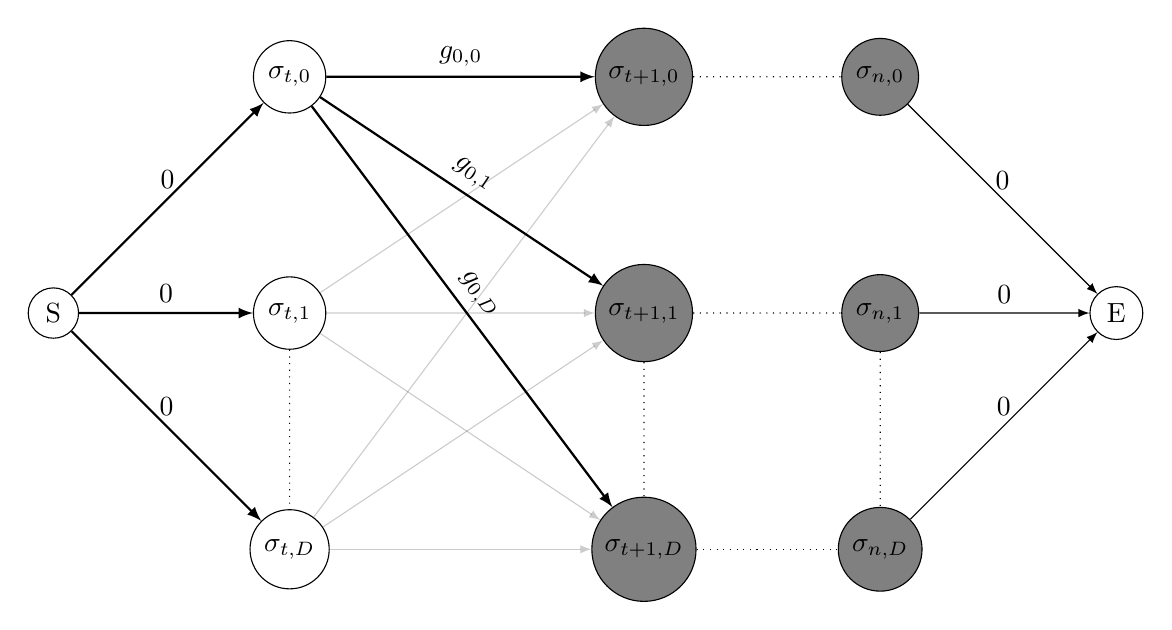
\begin{tikzpicture}[scale=1.5]
	\tikzstyle{vertex} = [circle, draw=black]
	\tikzstyle{vertex_closed_2} = [circle, draw=black, fill=gray, opacity = 30]
	\tikzstyle{vertex_opened} = [circle, draw=black]
	\tikzstyle{edge} = [->, thick]

%----------Виходить такий граф:------------------------------
	\node[vertex] (s) at (0,2) {S};
	
	\node[vertex] (v1n) at (2,0) {$\sigma_{t,D}$};
	\node[vertex] (v11) at (2,2) {$\sigma_{t,1}$};
	\node[vertex] (v10) at (2,4) {$\sigma_{t,0}$};
	
	\path[->, thick] (s) edge node[ above ] {0} (v1n);
	\path[->, thick] (s) edge node[ above ] {0} (v11);
	\path[->, thick] (s) edge node[ above ] {0} (v10);
	
	\draw[dash pattern=on \pgflinewidth off 2pt] (v11)--(v1n);
	
%------------------------------------------------------------
	\node[vertex_closed_2] (v2n) at (5,0) {$\sigma_{t+1,D}$};
	\node[vertex_closed_2] (v21) at (5,2) {$\sigma_{t+1,1}$};
	\node[vertex_closed_2] (v20) at (5,4) {$\sigma_{t+1,0}$};

	\path[->, opacity=0.2] (v11) edge node[ above,sloped ] {} (v2n);
	\path[->, opacity=0.2] (v11) edge node[ above,sloped ] {} (v21);
	\path[->, opacity=0.2] (v11) edge node[ above,sloped ] {} (v20);
	
	\path[->, opacity=0.2] (v1n) edge node[ above,sloped ] {} (v2n);
	\path[->, opacity=0.2] (v1n) edge node[ above,sloped ] {} (v21);
	\path[->, opacity=0.2] (v1n) edge node[ above,sloped ] {} (v20);
	
	%Selected
	\path[->, thick] (v10) edge node[ above,sloped ] {$g_{0,D}$} (v2n);
	\path[->, thick] (v10) edge node[ above,sloped ] {$g_{0,1}$} (v21);
	\path[->, thick] (v10) edge node[ above,sloped ] {$g_{0,0}$} (v20);
	
	\draw[dash pattern=on \pgflinewidth off 2pt] (v21)--(v2n);
	
	
%------------------------------------------------------------
	\node[vertex_closed_2] (vnn) at (7,0) {$\sigma_{n,D}$};
	\node[vertex_closed_2] (vn1) at (7,2) {$\sigma_{n,1}$};
	\node[vertex_closed_2] (vn0) at (7,4) {$\sigma_{n,0}$};


	\draw[dash pattern=on \pgflinewidth off 2pt] (v2n)--(vnn);
	\draw[dash pattern=on \pgflinewidth off 2pt] (v21)--(vn1);
	\draw[dash pattern=on \pgflinewidth off 2pt] (v20)--(vn0);
	
	\draw[dash pattern=on \pgflinewidth off 2pt] (vn1)--(vnn);
%------------------------------------------------------------
	\node[vertex] (e) at (9,2) {E};

	\path[->] (vnn) edge node[ above ] {0} (e);
	\path[->] (vn1) edge node[ above ] {0} (e);
	\path[->] (vn0) edge node[ above ] {0} (e);
	
	\end{tikzpicture}
	\caption{Граф $G$ }
	\label{graphG-2}
\end{figure}

Перед тим, як навести сам алгоритм, неформально опишемо ідею його роботи.
Припустимо, нам відомо, що найкоротший шлях з $S$ в $E$ проходить через вершину $ \sigma(t+1, d), d \in D $. 
Тоді, якщо всі вершини $ \sigma(t, d), \forall d \in D $ відкриті, ми можемо точно сказати, через яку з них буде проходити найкоротший шлях. На жаль, ми не знаємо, через яку вершину $ \sigma(t+1, d), d \in D $ буде проходити найкоротший шлях, тож нам необхідно для кожної такої вершини знайти її <<оптимальну попередню>> вершину. Зате після цього нам вже не потрібні вершини $ \sigma(t, d), \forall d \in D $, і ми можемо їх відкинути разом з їх ребрами, замінивши на $D_{max}$ нових ребер.
Цим самим ми зменшимо загальну кількість ребер на ${D_{max}}^2$.

Нехай $G^0 = <\mathcal{V}^0, \mathcal{E}^0> = <\mathcal{V}, \mathcal{E}> = G $. Нехай також $ T = \{1, ..., n-1\} $ --- множина ітерацій, $ s: T \times D \rightarrow R $, $s^0(d) = 0, \; \forall d \in D $. Для відновлення послідовності 
$\overline{d}$ введемо матрицю <<\textit{попередніх оптимальних вершин}>> $\hat{\mathcal{P}}$, розмірності $n \times (D_{max} + 1)$.  $$p_{1,d} = 0, \forall d \in D. $$

Як тільки автомат на кроці $ t \in T $ генерує нову пару $<cL, \;cR>$, шукаємо новий граф $G^t$:
\begin{enumerate}
	\item 
		$\forall d \in D :$\\
		$s^t(d) = \min\limits_{d' \in D} \big( s^{(t-1)}(d') + h(t, d') + g(d', d) \big).$\\
		$p_{t+1,d} = \argmin\limits_{d' \in D}{\big( s^{(t-1)}(d') + h(t, d') + g(d', d) \big) }$.
		(функція $ \argmin $ може повернути множину елементів, нам підходить будь-який з них)
	\item 
		$\mathcal{V}^t = \mathcal{V}^{t-1} \setminus \{ \sigma(t, d) \; | \; d \in D \}.$
	\item %\begin{align*}
		Позначимо множину $ \bigcup\limits_{d \in D} <S, \sigma(t, d) > $ як $ \mathcal{A},$ \\
		множину $ \bigcup\limits_{\substack{d \in D \\ d' \in D}} <\sigma(t, d), \sigma(t+1, d') > $ як $ \mathcal{B},$ \\
		а множину $ \bigcup\limits_{d \in D} <S, \sigma(t+1, d) > $ як $ \mathcal{C}. $ Тоді 
		$$\mathcal{E}^t = \Big( \mathcal{E}^{t-1} \setminus \big( \mathcal{A} \cup \mathcal{B} \big) \Big) \cup \mathcal{C}.$$
		Вага ребра $ <S, \sigma(t+1, d) > = s^t(d)$ %, \; \forall d \in D$.
		%\end{align*}
	\item 
		$G^t = <\mathcal{V}^t, \mathcal{E}^t> $ \\
\end{enumerate}

Коли ж на кроці $ n $ автомат згенерує останні пікселі зображень, нам залишиться тільки знайти
$$ d_n = \argmin\limits_{d' \in D} \big\{ { s^{(n-D_{max}-1)}(d') + h(n, d') } \big\},$$
та відновити послідовність $\overline{d}$ через матрицю $\hat{\mathcal{P}}$:
$$ d_i = p_{i+1,d_{i+1}}, i = \overline{n-1, 1}. $$

Кожен новий граф $G^t$ матиме на $(D_{max})^2$ менше ребер, ніж граф $G^{t-1}$. Таким чином, на момент приходу останніх пікселів, нам треба буде опрацювати лише $D_{max}$ ребер. А якщо б ми спочатку чекали приходу всіх даних, а тільки потім починали обчислення, нам треба було опрацювати 
$(n-1)(D_{max})^2$ ребер.

%%---------------------------------------------------------------------------%%
\subsection{Неупорядковане надходження даних при одному відомому зображені}
Нехай на початку нам відомі всі пікселі лише одного з зображень (рис. \ref{1.3nodata}).
\begin{figure}[h!]
	\centering
	\includegraphics[scale = 0.8]{allclosed.pdf}
	\caption{Немає даних}
	\label{1.3nodata}
\end{figure}
Введемо деякий стохастичний автомат, що на кожному кроці $ t \in I $ генерує пари $<i, \;c>$, де $ c $ --- інтенсивність пікселя з координатою $ i $ для невідомого зображення ($ i \in I, c \in \mathbb{R} $).
Тоді на кожному кроці $ t $ нам буде відкриватися стовпчик вершин $  h(i, d), \forall d \in D $ (рис. \ref{graphG-2}).
\begin{figure}[h!]
	\centering
	\tikzset{>=latex}
	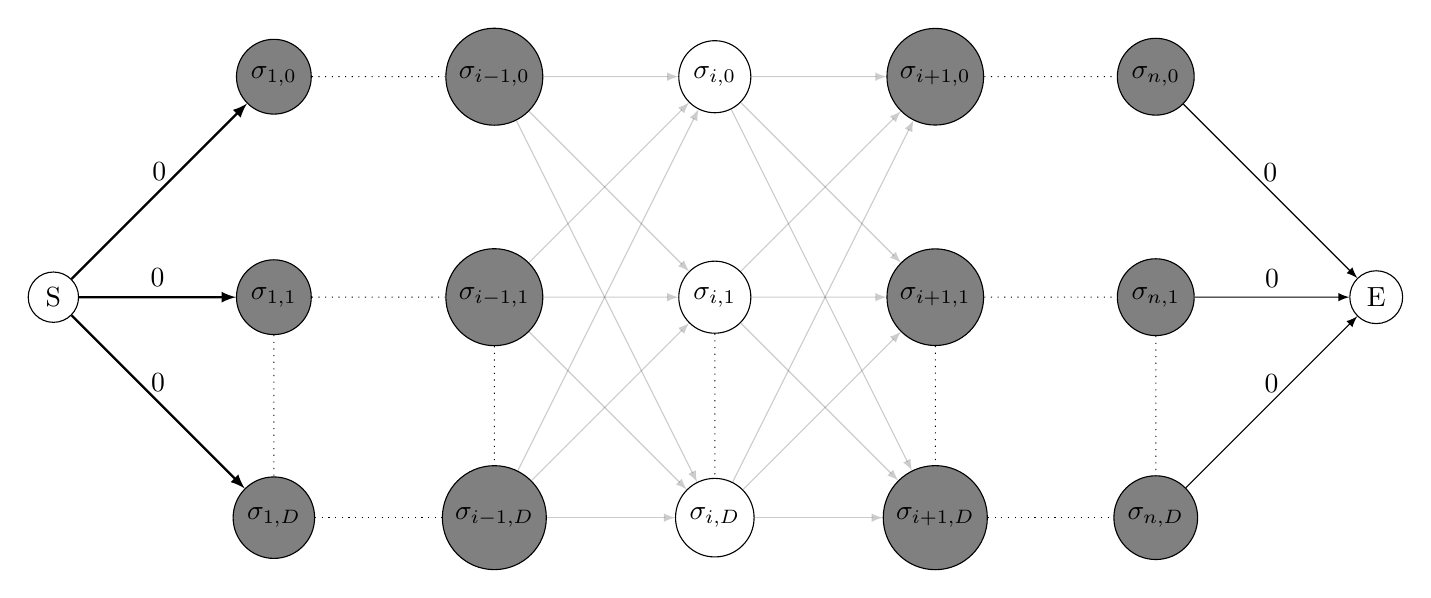
\begin{tikzpicture}[scale=1.4]
	\tikzstyle{vertex} = [circle, draw=black]
	\tikzstyle{vertex_closed_2} = [circle, draw=black, fill=gray, opacity = 30]
	\tikzstyle{vertex_opened} = [circle, draw=black]
	\tikzstyle{edge} = [->, thick]

%----------Виходить такий граф:------------------------------
	\node[vertex] (s) at (0,2) {S};
	
	\node[vertex_closed_2] (v1n) at (2,0) {$\sigma_{1,D}$};
	\node[vertex_closed_2] (v11) at (2,2) {$\sigma_{1,1}$};
	\node[vertex_closed_2] (v10) at (2,4) {$\sigma_{1,0}$};
	
	\path[->, thick] (s) edge node[ above ] {0} (v1n);
	\path[->, thick] (s) edge node[ above ] {0} (v11);
	\path[->, thick] (s) edge node[ above ] {0} (v10);
	
	\draw[dash pattern=on \pgflinewidth off 2pt] (v11)--(v1n);
	
%------------------------------------------------------------
	\node[vertex_closed_2] (v2n) at (4,0) {$\sigma_{i-1,D}$};
	\node[vertex_closed_2] (v21) at (4,2) {$\sigma_{i-1,1}$};
	\node[vertex_closed_2] (v20) at (4,4) {$\sigma_{i-1,0}$};

	\draw[dash pattern=on \pgflinewidth off 2pt] (v10)--(v20);
	\draw[dash pattern=on \pgflinewidth off 2pt] (v11)--(v21);
	\draw[dash pattern=on \pgflinewidth off 2pt] (v1n)--(v2n);
	
	\draw[dash pattern=on \pgflinewidth off 2pt] (v21)--(v2n);
	
	
%------------------------------------------------------------
	\node[vertex_opened] (v3n) at (6,0) {$\sigma_{i,D}$};
	\node[vertex_opened] (v31) at (6,2) {$\sigma_{i,1}$};
	\node[vertex_opened] (v30) at (6,4) {$\sigma_{i,0}$};

	\path[->, opacity=0.2] (v21) edge node[ above,sloped ] {} (v3n);
	\path[->, opacity=0.2] (v21) edge node[ above,sloped ] {} (v31);
	\path[->, opacity=0.2] (v21) edge node[ above,sloped ] {} (v30);
	
	\path[->, opacity=0.2] (v2n) edge node[ above,sloped ] {} (v3n);
	\path[->, opacity=0.2] (v2n) edge node[ above,sloped ] {} (v31);
	\path[->, opacity=0.2] (v2n) edge node[ above,sloped ] {} (v30);
	
	\path[->, opacity=0.2] (v20) edge node[ above,sloped ] {} (v3n);
	\path[->, opacity=0.2] (v20) edge node[ above,sloped ] {} (v31);
	\path[->, opacity=0.2] (v20) edge node[ above,sloped ] {} (v30);
	
	\draw[dash pattern=on \pgflinewidth off 2pt] (v31)--(v3n);

%------------------------------------------------------------
	\node[vertex_closed_2] (v4n) at (8,0) {$\sigma_{i+1,D}$};
	\node[vertex_closed_2] (v41) at (8,2) {$\sigma_{i+1,1}$};
	\node[vertex_closed_2] (v40) at (8,4) {$\sigma_{i+1,0}$};

	\path[->, opacity=0.2] (v31) edge node[ above,sloped ] {} (v4n);
	\path[->, opacity=0.2] (v31) edge node[ above,sloped ] {} (v41);
	\path[->, opacity=0.2] (v31) edge node[ above,sloped ] {} (v40);
	
	\path[->, opacity=0.2] (v3n) edge node[ above,sloped ] {} (v4n);
	\path[->, opacity=0.2] (v3n) edge node[ above,sloped ] {} (v41);
	\path[->, opacity=0.2] (v3n) edge node[ above,sloped ] {} (v40);
	
	\path[->, opacity=0.2] (v30) edge node[ above,sloped ] {} (v4n);
	\path[->, opacity=0.2] (v30) edge node[ above,sloped ] {} (v41);
	\path[->, opacity=0.2] (v30) edge node[ above,sloped ] {} (v40);
	
	\draw[dash pattern=on \pgflinewidth off 2pt] (v41)--(v4n);

%------------------------------------------------------------
	\node[vertex_closed_2] (vnn) at (10,0) {$\sigma_{n,D}$};
	\node[vertex_closed_2] (vn1) at (10,2) {$\sigma_{n,1}$};
	\node[vertex_closed_2] (vn0) at (10,4) {$\sigma_{n,0}$};


	\draw[dash pattern=on \pgflinewidth off 2pt] (v4n)--(vnn);
	\draw[dash pattern=on \pgflinewidth off 2pt] (v41)--(vn1);
	\draw[dash pattern=on \pgflinewidth off 2pt] (v40)--(vn0);
	
	\draw[dash pattern=on \pgflinewidth off 2pt] (vn1)--(vnn);
	
%------------------------------------------------------------
	\node[vertex] (e) at (12,2) {E};

	\path[->] (vnn) edge node[ above ] {0} (e);
	\path[->] (vn1) edge node[ above ] {0} (e);
	\path[->] (vn0) edge node[ above ] {0} (e);
	
	\end{tikzpicture}
	\caption{Граф $G$ (відкриті вершини зафарбовані білим). }
	\label{graphG-2}
\end{figure}

Перед тим як навести сам алгоритм, неформально опишемо ідею його роботи.
Припустимо, нам відомо, що найкоротший шлях з $S$ в $E$ проходить через 
вершини $ \sigma(i+1, d')$ та $\sigma(i-1,d''), \; d', d'' \in D, i \in I $. 
Коли вершини $ \sigma(i, d), \; \forall d \in D $ стають відкритими, ми можемо точно сказати, через яку з них буде він буде проходити. Проте, $ d'$ та $ d'' $ нам не відомі, тому нам необхідно для кожної пари вершини 
$ \sigma(i-1, d')$ та $  \sigma(i+1, d'') $ знайти їх <<оптимальну середню>> вершину. 
Після цього вершини $ \sigma(i, d), \forall d \in D $ нам вже не потрібні, і ми можемо їх відкинути разом з їх ребрами, замінивши на ${D_{max}}^2$ нових ребер, зменшивши загальну кількість ребер теж на ${D_{max}}^2$. 

Покладемо $G^0 = <\mathcal{V}^0, \mathcal{E}^0> = <\mathcal{V}, \mathcal{E}> = G.$
Також $ T = \{1, ..., n-1\} $ --- множина ітерацій. На кожній ітерації $ t $ будемо замінювати граф $ G^{t-1} $ на новий граф $ G^t $, що буде мати менше ребер та вершин. Введемо також функцію 
$$ w : T \times E \rightarrow \mathbb{R} ,$$
де $ w^t(v_1, v_2) $ --- вага ребра $ <v_1, v_2> $ у графі $ G^t \; (<v_1, v_2> \in E^t )$. Для знаходження cусідніх стовпчиків закритих вершин у графі $ G^t $ вводимо
$$ j = i - \sum\limits_{k = 1}^{i}{ \mathds{1}(\mathcal{L}(k) \neq \varepsilon ) }$$
Для відновлення послідовності $\overline{d}$ введемо матрицю <<\textit{оптимальних вершин}>> $\hat{\mathcal{P}}$, розмірності $I \times {(D_{max} + 1)} \times {(D_{max} + 1)}$, та покладемо 
$${p^i}_{d',d''} = 0, \; \forall d',d'' \in D, \forall i \in I. $$

\newpage

Як тільки автомат на кроці $ t \in T $ генерує нову пару $<i, \;c>$, шукаємо новий граф $G^t$:
\begin{enumerate}
	\item
		$ j = i - \sum\limits_{k = 1}^{i}{ \mathds{1}(\mathcal{L}(k) \neq \varepsilon ) } $,\\
		$ \hat{n} = n - \sum\limits_{k = 1}^{n}{ \mathds{1}(\mathcal{L}(k) \neq \varepsilon ) } $.\\
	\item 
		якщо $ j = 0$:\\
		$ w^t(s, \sigma(j+1, d)) = \min\limits_{\hat{d} \in D} 
		\big( w^{t-1}(s, \sigma(i,\hat{d})) + h(i, \hat{d}) +  w^{t-1}(\sigma(i, \hat{d}), \sigma(j+1,d)) \big), $ \\
		
		$ {p^i}_{d',d''} = \argmin\limits_{\hat{d} \in D} 
		\big( w^{t-1}(s, \sigma(i,\hat{d})) + h(i, \hat{d}) +  w^{t-1}(\sigma(i, \hat{d}), \sigma(j+1,d)) \big). $\\
	\item 
		якщо $ j = \hat{n}$:\\
		
		$ w^t(\sigma(j, d) , e ) = \min\limits_{\hat{d} \in D} 
		\big( w^{t-1}(\sigma(j, d), \sigma(i,\hat{d})) + h(i, \hat{d}) +  w^{t-1}(\sigma(i, \hat{d}), e) \big), $ \\
		
		$ {p^i}_{d',d''} = \argmin\limits_{\hat{d} \in D} 
		\big( w^{t-1}(\sigma(j, d), \sigma(i,\hat{d})) + h(i, \hat{d}) +  w^{t-1}(\sigma(i, \hat{d}), e) \big). $  \\
	\item 
		якщо $ 0 < j < \hat{n}$:\\
		
		$ w^t(\sigma(j, d') , \sigma(j+1, d'') ) = \min\limits_{\hat{d} \in D} 
		\Big( w^{t-1}(\sigma(j, d'), \sigma(i,\hat{d})) + h(i, \hat{d}) + $\\
		$+  w^{t-1}(\sigma(i, \hat{d}), \sigma(j+1, d'') \Big), $ \\
		
		$ {p^i}_{d',d''} = \argmin\limits_{\hat{d} \in D} 
		\Big( w^{t-1}(\sigma(j, d'), \sigma(i,\hat{d})) +  h(i, \hat{d}) +  w^{t-1}(\sigma(i, \hat{d}), \sigma(j+1, d'') \Big). $  \\
	\item 
		$\mathcal{V}^t = \mathcal{V}^{t-1} \setminus \{ \sigma(i, d) \; | \; \forall d \in D \}.$\\
	\item %\begin{align*}
		Позначимо множину $ \bigcup\limits_{d \in D} <S, \sigma(i, d) > $ як $ \mathcal{A}(i),$ \\
		множину $ \bigcup\limits_{\substack{d \in D \\ d' \in D}} <\sigma(i, d), \sigma(i+1, d') > $ як $ \mathcal{B}(i),$ \\
		а множину $ \bigcup\limits_{d \in D} <S, \sigma(t+1, d) > $ як $ \mathcal{C}. $ Тоді 
		$$\mathcal{E}^t = \Big( \mathcal{E}^{t-1} \setminus \big( \mathcal{A} \cup \mathcal{B} \big) \Big) \cup \mathcal{C}.$$
		Вага ребра $ <S, \sigma(t+1, d) > = s^t(d)$ %, \; \forall d \in D$.
		%\end{align*}
	\item 
		$G^t = <\mathcal{V}^t, \mathcal{E}^t> $ \\
\end{enumerate}

Коли ж на кроці $ n $ автомат згенерує останні пікселі зображень, нам залишиться тільки знайти
$$ d_n = \argmin\limits_{d' \in D} \big\{ { s^{(n-D_{max}-1)}(d') + h(n, d') } \big\},$$
та відновити послідовність $\overline{d}$ через матрицю $\hat{\mathcal{P}}$:
$$ d_i = p_{i+1,d_{i+1}}, i = \overline{n-1, 1}. $$

Кожен новий граф $G^t$ матиме на $(D_{max})^2$ менше ребер, ніж граф $G^{t-1}$. Таким чином, на момент приходу останніх пікселів, нам треба буде опрацювати лише $D_{max}$ ребер. А якщо б ми спочатку чекали приходу всіх даних, а тільки потім починали обчислення, нам треба було опрацювати 
$(n-1)(D_{max})^2$ ребер.










%%===========================================================================%%
\section{Стереозрение при медленно поступающих данных}
%%===========================================================================%%
Описать что такое медленно приходящие данные...

%%-------------------------------------------------%%
\subsection{Данные приходят по порядку}
%%-------------------------------------------------%%
Пусть сначала все пиксели нам неизвестны (рис. \ref{1.4_im_nodata}), поэтому мы не можем вычислить вес ни одной из вершин графа $G$ ( \ref{Def_G}).
%2.1nodata
\begin{figure}[h!]
	\centering
	\includegraphics[scale = 0.7]{allclosed2.pdf}
	\caption{Нет данных}
	\label{1.4_im_nodata}
\end{figure}

\label {2.1-style} Если мы не можем вычислить вес вершины --- будем называть эту вершину ''\textit{закрытой}'' и обозначать ее черным кружочком. В противном случае назовем вершину ''\textit{открытой}'' и обозначим белым кружком. Для простоты рисунков положим $ D_{max} = 2 $ и не будем обозначать ребер. Тогда, в ситуации когда все данные нам неизвестны, граф $ G $ будет иметь следующий вид (рис. \ref{1.4Gnodata}). 
%Gnodata
\begin{figure}[h!]
	\centering
	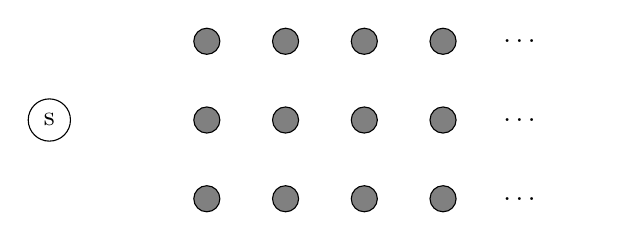
\begin{tikzpicture}[scale=1]
	\tikzstyle{vertex_closed_1} = [circle, draw=black, fill=gray, opacity=0.3]
	\tikzstyle{vertex_closed_2} = [circle, draw=black, fill=gray]
	\tikzstyle{vertex_opened} = [circle, draw=black]

%------------------------------------------------------------
	\node[vertex_opened] (s) at (-1,1) {s};

	\node[vertex_closed_2] (v00) at (1,0) {};
	\node[vertex_closed_2] (v01) at (1,1) {};
	\node[vertex_closed_2] (v02) at (1,2) {};
		
%------------------------------------------------------------
	
	\node[vertex_closed_2] (v10) at (2,0) {};
	\node[vertex_closed_2] (v11) at (2,1) {};
	\node[vertex_closed_2] (v12) at (2,2) {};
		
%------------------------------------------------------------
	
	\node[vertex_closed_2] (v20) at (3,0) {};
	\node[vertex_closed_2] (v21) at (3,1) {};
	\node[vertex_closed_2] (v22) at (3,2) {};
		
%------------------------------------------------------------
	
	\node[vertex_closed_2] (v30) at (4,0) {};
	\node[vertex_closed_2] (v31) at (4,1) {};
	\node[vertex_closed_2] (v32) at (4,2) {};
		
%------------------------------------------------------------

	\node[vertex_closed_2, opacity =0] (v40) at (6,0) {};
	\node[vertex_closed_2, opacity =0] (v41) at (6,1) {};
	\node[vertex_closed_2, opacity =0] (v42) at (6,2) {};
	
	\path (v30) -- node[auto=false]{\ldots} (v40);
	\path (v31) -- node[auto=false]{\ldots} (v41);
	\path (v32) -- node[auto=false]{\ldots} (v42);
	
	\end{tikzpicture}
	\captionof{figure}{граф $G$ в отсутствии данных}
	\label{1.4Gnodata}
\end{figure}

Пусть теперь нам по порядку начинают приходить пары из пикселей правого и левого изображений с одинаковыми координатами. Когда нам известен только один первый пиксель каждого изображения (рис.\ref{1.4_im_onepixel}) то мы можем вычислить вес только одной вершины, и граф $G$ будет иметь вид как на рис.\ref{1.4_pl_Gonepixel}.
%1.4_im_onepixel
\begin{figure}[h!]
	\centering
	\includegraphics[scale = 0.7]{onestereoknown.pdf}
	\caption{Известны только первые пиксели}
	\label{1.4_im_onepixel}
\end{figure}
%1.4_pl_Gonepixel
\begin{figure}[h!]
	\centering
	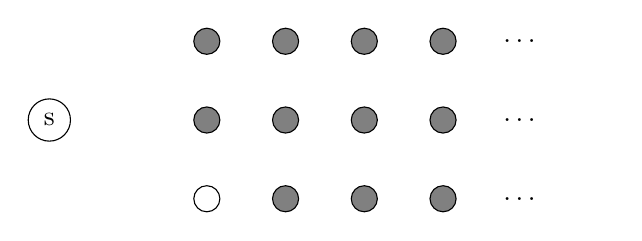
\begin{tikzpicture}[scale=1]

	\tikzstyle{vertex_closed_1} = [circle, draw=black, fill=gray, opacity=0.3]
	\tikzstyle{vertex_closed_2} = [circle, draw=black, fill=gray]
	\tikzstyle{vertex_opened} = [circle, draw=black]

%------------------------------------------------------------
	\node[vertex_opened] (s) at (-1,1) {s};

	\node[vertex_opened] (v00) at (1,0) {};
	\node[vertex_closed_2] (v01) at (1,1) {};
	\node[vertex_closed_2] (v02) at (1,2) {};
		
%------------------------------------------------------------
	
	\node[vertex_closed_2] (v10) at (2,0) {};
	\node[vertex_closed_2] (v11) at (2,1) {};
	\node[vertex_closed_2] (v12) at (2,2) {};
		
%------------------------------------------------------------
	
	\node[vertex_closed_2] (v20) at (3,0) {};
	\node[vertex_closed_2] (v21) at (3,1) {};
	\node[vertex_closed_2] (v22) at (3,2) {};
		
%------------------------------------------------------------
	
	\node[vertex_closed_2] (v30) at (4,0) {};
	\node[vertex_closed_2] (v31) at (4,1) {};
	\node[vertex_closed_2] (v32) at (4,2) {};
		
%------------------------------------------------------------

	\node[vertex_closed_2, opacity =0] (v40) at (6,0) {};
	\node[vertex_closed_2, opacity =0] (v41) at (6,1) {};
	\node[vertex_closed_2, opacity =0] (v42) at (6,2) {};
	
	\path (v30) -- node[auto=false]{\ldots} (v40);
	\path (v31) -- node[auto=false]{\ldots} (v41);
	\path (v32) -- node[auto=false]{\ldots} (v42);
	
	\end{tikzpicture}
	\captionof{figure}{Граф $G$ когда известны только первые пиксели}
	\label{1.4_pl_Gonepixel}
\end{figure}

Когда же нам будут известны уже первые два пикселя обоих изображений, мы сможем найти веса уже трёх вершин, и граф $G$ будет выглядеть как на рис.\ref{1.4_pl_twopixels}.
%G1.4_pl_twopixels
\begin{figure}[h!]
	\centering
	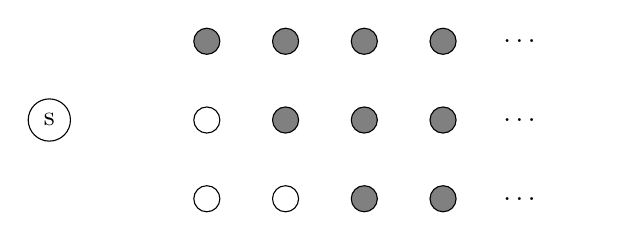
\begin{tikzpicture}[scale=1]
	\tikzstyle{vertex_closed_1} = [circle, draw=black, fill=gray, opacity=0.3]
	\tikzstyle{vertex_closed_2} = [circle, draw=black, fill=gray]
	\tikzstyle{vertex_opened} = [circle, draw=black]

%------------------------------------------------------------
	\node[vertex_opened] (s) at (-1,1) {s};

	\node[vertex_opened] (v00) at (1,0) {};
	\node[vertex_opened] (v01) at (1,1) {};
	\node[vertex_closed_2] (v02) at (1,2) {};
		
%------------------------------------------------------------
	
	\node[vertex_opened] (v10) at (2,0) {};
	\node[vertex_closed_2] (v11) at (2,1) {};
	\node[vertex_closed_2] (v12) at (2,2) {};
		
%------------------------------------------------------------
	
	\node[vertex_closed_2] (v20) at (3,0) {};
	\node[vertex_closed_2] (v21) at (3,1) {};
	\node[vertex_closed_2] (v22) at (3,2) {};
		
%------------------------------------------------------------
	
	\node[vertex_closed_2] (v30) at (4,0) {};
	\node[vertex_closed_2] (v31) at (4,1) {};
	\node[vertex_closed_2] (v32) at (4,2) {};
		
%------------------------------------------------------------

	\node[vertex_closed_2, opacity =0] (v40) at (6,0) {};
	\node[vertex_closed_2, opacity =0] (v41) at (6,1) {};
	\node[vertex_closed_2, opacity =0] (v42) at (6,2) {};
	
	\path (v30) -- node[auto=false]{\ldots} (v40);
	\path (v31) -- node[auto=false]{\ldots} (v41);
	\path (v32) -- node[auto=false]{\ldots} (v42);
	
	\end{tikzpicture}
	\captionof{figure}{Відомі перші два пікселі зображень}
	\label{1.4_pl_twopixels}
\end{figure}

По мере прихода следующих пикселей в графе $G$ будут открываться вершины на диагонали над уже открытыми вершинами. А как только нам станут известны $D_{max} + 1$ первых пикселей обоих изображений --- то все вершины в первом столбике станут открытыми (рис. \ref{1.4_pl_Dpixels}), и мы можем приступать к предвычислениям  
%1.4_pl_Dpixels
\begin{figure}[h!]
	\centering
	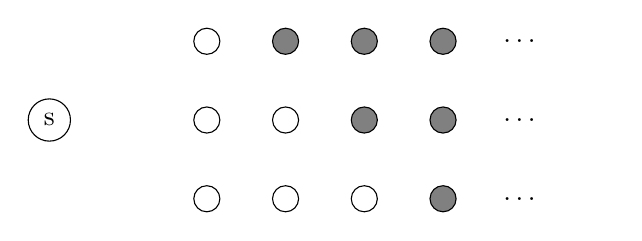
\begin{tikzpicture}[scale=1]

	\tikzstyle{vertex_closed_1} = [circle, draw=black, fill=gray, opacity=0.3]
	\tikzstyle{vertex_closed_2} = [circle, draw=black, fill=gray]
	\tikzstyle{vertex_opened} = [circle, draw=black]

%------------------------------------------------------------
	\node[vertex_opened] (s) at (-1,1) {s};

	\node[vertex_opened] (v00) at (1,0) {};
	\node[vertex_opened] (v01) at (1,1) {};
	\node[vertex_opened] (v02) at (1,2) {};
		
%------------------------------------------------------------
	
	\node[vertex_opened]   (v10) at (2,0) {};
	\node[vertex_opened]   (v11) at (2,1) {};
	\node[vertex_closed_2] (v12) at (2,2) {};
		
%------------------------------------------------------------
	
	\node[vertex_opened]   (v20) at (3,0) {};
	\node[vertex_closed_2] (v21) at (3,1) {};
	\node[vertex_closed_2] (v22) at (3,2) {};
		
%------------------------------------------------------------
	
	\node[vertex_closed_2] (v30) at (4,0) {};
	\node[vertex_closed_2] (v31) at (4,1) {};
	\node[vertex_closed_2] (v32) at (4,2) {};
		
%------------------------------------------------------------

	\node[vertex_closed_2, opacity =0] (v40) at (6,0) {};
	\node[vertex_closed_2, opacity =0] (v41) at (6,1) {};
	\node[vertex_closed_2, opacity =0] (v42) at (6,2) {};
	
	\path (v30) -- node[auto=false]{\ldots} (v40);
	\path (v31) -- node[auto=false]{\ldots} (v41);
	\path (v32) -- node[auto=false]{\ldots} (v42);
	
	\end{tikzpicture}
	\captionof{figure}{Известны первые $D_{max} + 1$ пікселей}
	\label{1.4_pl_Dpixels}
\end{figure}
\newpage

Предположим кратчайший путь проходит через какую-то вершину $\sigma(2, d)$ во втором столбике. Тогда точно можно утверждать, что он проходит через вершину 
$\sigma(1, k)$ первого столбика, где 
$$k = \argmin\limits_{l=0}^{D_{max}}{\big( h(1, l) + g(l, d) \big) }.$$
Тогда все остальные возможные пути из $S$ в $\sigma(2, d)$ нам не нужны, и мы их отбрасываем, а вместо них вводим ребро $<S, \sigma(2, d) >$, с весом 
$${g^{(1)}}_d = \min\limits_{l=0}^{D_{max}}{\big( h(2, l) + g(l, d) \big) },  \; \forall d \in D.$$ 
Таким образом мы уменьшили количество рёбер в графе $G$ на $D_{max}$.
 
Но мы не знаем через какую именно вершину второго столбика проходит кратчайший путь, поэтому вынуждены провести эту операцию для всех вершин $\sigma(2, d) \; \forall d \in D$.В результате такой оптимизации мы сократим количество рёбер на $(D_{max})^2$ (рис. \ref{1.4_pl_notoptimized} $\rightarrow$ рис. \ref{1.4_pl_optimized}).
%1.4_pl_notoptimized
\begin{figure}[h!]
	\centering
	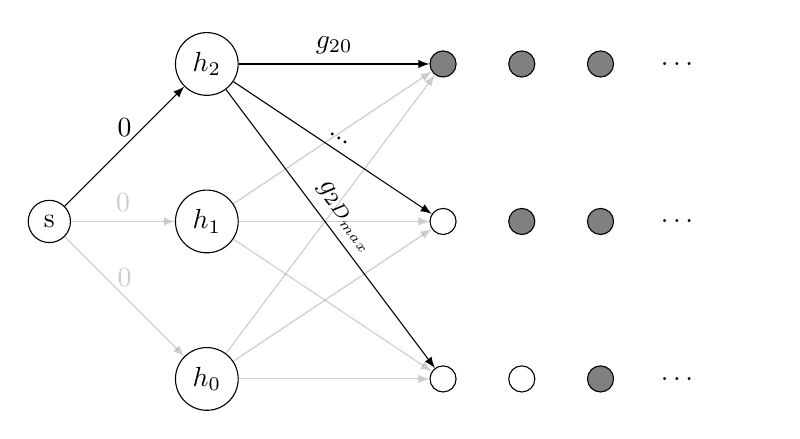
\begin{tikzpicture}[scale=1]

	\tikzstyle{vertex_closed_1} = [circle, draw=black, fill=gray] %opacity=0.3]
	\tikzstyle{vertex_closed_2} = [circle, draw=black, fill=gray]
	\tikzstyle{vertex_opened} = [circle, draw=black]

%------------------------------------------------------------
	\node[vertex_opened] (s) at (-2,2) {s};

	\node[vertex_opened] (v00) at (0,0) {$h_0$};
	\node[vertex_opened] (v01) at (0,2) {$h_1$};
	\node[vertex_opened] (v02) at (0,4) {$h_2$};
	
	\path[-latex, opacity=1]   (s) edge node[ above ] {$0$} (v02);
	\path[-latex, opacity=0.2] (s) edge node[ above ] {$0$} (v01);
	\path[-latex, opacity=0.2] (s) edge node[ above ] {$0$} (v00);
		
%------------------------------------------------------------
	
	\node[vertex_opened]   (v10) at (3,0) {};
	\node[vertex_opened]   (v11) at (3,2) {};
	\node[vertex_closed_1] (v12) at (3,4) {};
		
	\path[-latex, opacity=1] (v02) edge node[ sloped, above ] {$g_{2D_{max}}$} (v10);
	\path[-latex, opacity=1] (v02) edge node[ sloped, above ] {$...$} (v11);
	\path[-latex, opacity=1] (v02) edge node[ sloped, above ] {$g_{20}$} (v12);
	
	\path[-latex, opacity=0.2] (v01) edge node[ above ] {} (v10);
	\path[-latex, opacity=0.2] (v01) edge node[ above ] {} (v11);
	\path[-latex, opacity=0.2] (v01) edge node[ above ] {} (v12);
	
	\path[-latex, opacity=0.2] (v00) edge node[ above ] {} (v10);
	\path[-latex, opacity=0.2] (v00) edge node[ above ] {} (v11);
	\path[-latex, opacity=0.2] (v00) edge node[ above ] {} (v12);
%------------------------------------------------------------
	
	\node[vertex_opened]   (v20) at (4,0) {};
	\node[vertex_closed_1] (v21) at (4,2) {};
	\node[vertex_closed_1] (v22) at (4,4) {};
		
%------------------------------------------------------------
	
	\node[vertex_closed_1] (v30) at (5,0) {};
	\node[vertex_closed_1] (v31) at (5,2) {};
	\node[vertex_closed_1] (v32) at (5,4) {};
		
%------------------------------------------------------------

	\node[vertex_closed_1, opacity =0] (v40) at (7,0) {};
	\node[vertex_closed_1, opacity =0] (v41) at (7,2) {};
	\node[vertex_closed_1, opacity =0] (v42) at (7,4) {};
	
	\path (v30) -- node[auto=false]{\ldots} (v40);
	\path (v31) -- node[auto=false]{\ldots} (v41);
	\path (v32) -- node[auto=false]{\ldots} (v42);
	
	\end{tikzpicture}
	\captionof{figure}{граф $G$ до оптимизации}
	\label{1.4_pl_notoptimized}
\end{figure}
%1.4_pl_optimized
\begin{figure}[h!]
	\centering
	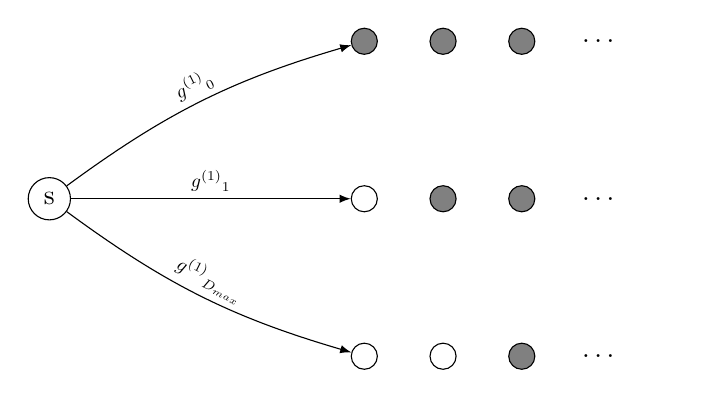
\begin{tikzpicture}[scale=1]
	\tikzstyle{vertex_closed_1} = [circle, draw=black, fill=gray]
	\tikzstyle{vertex_closed_2} = [circle, draw=black, fill=gray]
	\tikzstyle{vertex_opened} = [circle, draw=black]

%------------------------------------------------------------
	\node[vertex_opened] (s) at (-2,2) {s};
	
	\node[vertex_opened]   (v10) at (2,0) {};
	\node[vertex_opened]   (v11) at (2,2) {};
	\node[vertex_closed_1] (v12) at (2,4) {};
		
	\path[-latex, opacity=1]   (s) edge[bend right=10] node[ above, sloped, scale = 0.7 ] {${g^{(1)}}_{D_{max}}$} (v10);
	\path[-latex, opacity=1]   (s) edge node[ above, sloped, scale = 0.7 ] {${g^{(1)}}_1$} (v11);
	\path[-latex, opacity=1]   (s) edge[bend right=-10] node[ above, sloped, scale = 0.7 ] {${g^{(1)}}_0$} (v12);
%------------------------------------------------------------
	
	\node[vertex_opened]   (v20) at (3,0) {};
	\node[vertex_closed_1] (v21) at (3,2) {};
	\node[vertex_closed_1] (v22) at (3,4) {};
		
%------------------------------------------------------------
	
	\node[vertex_closed_1] (v30) at (4,0) {};
	\node[vertex_closed_1] (v31) at (4,2) {};
	\node[vertex_closed_1] (v32) at (4,4) {};
		
%------------------------------------------------------------

	\node[vertex_closed_1, opacity =0] (v40) at (6,0) {};
	\node[vertex_closed_1, opacity =0] (v41) at (6,2) {};
	\node[vertex_closed_1, opacity =0] (v42) at (6,4) {};
	
	\path (v30) -- node[auto=false]{\ldots} (v40);
	\path (v31) -- node[auto=false]{\ldots} (v41);
	\path (v32) -- node[auto=false]{\ldots} (v42);
	
	\end{tikzpicture}
	\captionof{figure}{граф $G$ после оптимизации}
	\label{1.4_pl_optimized}
\end{figure}	
\newpage

По пришествию первых $D_{max} + 2$ стерео-пар пикселей проводим аналогичные действия, но теперь уже учитываем предыдущую оптимизацию. Для каждой вершины $\sigma(3, d) \; d \in D$ находим вершину $\sigma(2, k)$, где 
$$ k = \argmin\limits_{l \in D}{\big( g^{(1)}_l +  h(2, l) + g(l, d) \big) }. $$
Отбрасываем все пути из $S$ в $\sigma(3, d), \; d \in D $, и вводим рёбра $<S, \sigma(3, d) >  \; d \in D$ c весами 
$${g^{(2)}}_d = \min\limits_{l \in D}{\big( g^{(1)}_l + h(2, l) + g(l, d) \big) },  \; \forall d \in D.$$
Этим самым снова уменьшив общее количество рёбер графа $G$ на $(D_{max})^2$.

Таким образом, при как только становятся известны первые $D_{max}+m$ стерео-пар пикселей $( m \geqslant 2)$, отбрасываем все пути из $S$ в 
$\sigma(m+1, d) \; d \in D$, заменяя их рёбрами $<S, \sigma(m+1, d) > \; \forall d \in D$, с весами 
\begin{equation}\label{1.4_f_g^i}
{g^{(m)}}_d = \min\limits_{l \in D}{\big( g^{(m-1)}_l + h(m, l) + g(l, d) \big) },  \; \forall d \in D,
\end{equation}
уменьшая количество рёбер графа $G$ ещё на $(D_{max})^2$.
\newpage

Для восстановления конечной оптимальной последовательности $\overline{d}$, нам для каждой вершины $\sigma(i, d), \; \forall \;	i = \overline{2, n}, \; d \in D$ нужно запоминать предыдущую ей ''\textit{оптимальную}'' вершину $\sigma(i-1, k)$, где 
%\begin{equation}\label{1.4_f_k}
$$k = \argmin\limits_{l \in D}{\big( {g^{(i-1)}}_l + h(i-1, l) + g(l, d) \big) }.$$
Для этого введем матрицу предыдущих оптимальных вершин $\hat{\mathcal{P}}$ размера \\
$n \times D_{max} + 1$, где $\sigma(i-1, p_{ij}) $ --- предыдущая $\sigma(i, j)$ оптимальная вершина, \\
$\forall i \in I, j \in D$. Элементы этой матрицы находятся следующим образом:
\begin{itemize}
\item $p_{1j} = 0, \; \forall j \in D$ поскольку в вершины первого столбца можно попасть только из начальной вершины $S$, и предыдущая оптимальная вершина для них всегда одна. Конечно, можно просто исключить эти элементы из матрицы, но их наличие приводит к более красивому и простому определению остальных элементов матрицы 
$\hat{\mathcal{P}}$.
\item $p_{ij} = \argmin\limits_{l \in D}{\big( {g^{(i-1)}}_l + h(i-1, l) + g(l, j) \big) }.$
\end{itemize}
Элементы $p_{ij}$ нужно вычислять при приходе $D_{max} + i$ пары пикселей, так как при приходе следующей пары, рёбра $ g^{(i-1)}_l $ используются  
для расчёта рёбер $ g^{(i)}_l, \; \forall l \in D $ согласно формуле \ref{1.4_f_g^i} и отбрасываются.

После нахождения всех элементов $\hat{\mathcal{P}}$, можем восстановить все элементы последовательности $\overline{d}$ ---
\begin{align*}
d_n &= \argmin\limits_{l \in D}  {\big( {g^{(n-1)}}_l + h(n, l) \big) }, \\
d_{n-1} &= p_{n,d_n},\\
&\cdots\\
d_i &= p_{i,d_{n-1}}.
\end{align*}



%%-------------------------------------------------%%
\subsection{Одно из изображений известно}
%%-------------------------------------------------%%

























